\documentclass[12pt, a4paper, oneside]{ctexart}
\usepackage{amsmath, amsthm, amssymb, bm, color, graphicx, geometry, mathrsfs,extarrows, braket, booktabs, array}
\usepackage[colorlinks,linkcolor=red,anchorcolor=blue,citecolor=blue,urlcolor=blue,menucolor=black]{hyperref}
\setCJKmainfont{方正新书宋_GBK.ttf}[ BoldFont = 方正小标宋_GBK, ItalicFont = 方正楷体_GBK]
\setmainfont{Times New Roman}  % 设置英文字体
\setsansfont{Calibri}
\setmonofont{Consolas}

\linespread{1.4}
%\geometry{left=2.54cm,right=2.54cm,top=3.18cm,bottom=3.18cm}
\geometry{left=1.84cm,right=1.84cm,top=2.18cm,bottom=2.18cm}
\newcounter{problem}  % 问题序号计数器
\newenvironment{problem}{\stepcounter{problem}\par\noindent\textbf{题目\arabic{problem}. }}{\smallskip\par}
\newenvironment{solution}{\par\noindent\textbf{解答. }}{\smallskip\par}
\newenvironment{note}{\par\noindent\textbf{注记. }}{\smallskip\par}

%%%% 图片相对路径 %%%%
\graphicspath{{figure/}} % 当前目录下的figure文件夹, {../figure/}则是父目录的figure文件夹

\everymath{\displaystyle} % 默认全部行间公式
\DeclareMathOperator*\uplim{\overline{lim}} % 定义上极限 \uplim_{}
\DeclareMathOperator*\lowlim{\underline{lim}} % 定义下极限 \lowlim_{}
\let\leq=\leqslant % 将全部leq变为leqslant
\let\geq=\geqslant % geq同理

%%%% 一些宏定义 %%%%
\def\bd{\boldsymbol}        % 加粗(向量) boldsymbol
\def\disp{\displaystyle}    % 使用行间公式 displaystyle(默认)
\def\tsty{\textstyle}       % 使用行内公式 textstyle
\def\sign{\text{sign}}      % sign function
\def\wtd{\widetilde}        % 宽波浪线 widetilde
\def\R{\mathbb{R}}          % Real number
\def\N{\mathbb{N}}          % Natural number
\def\Z{\mathbb{Z}}          % Integer number
\def\Q{\mathbb{Q}}          % Rational number
\def\C{\mathbb{C}}          % Complex number
\def\d{\mathrm{d}}          % differential operator
\def\e{\mathrm{e}}          % Euler's number
\def\i{\mathrm{i}}          % imaginary number
\def\re{\mathrm{Re}}        % Real part
\def\im{\mathrm{Im}}        % Imaginary part
\def\res{\mathrm{Res}}      % Residue
\def\L{\mathcal{L}}         % Loss function
\def\wdh{\widehat}          % 宽帽子 widehat
\def\ol{\overline}          % 上横线 overline
\def\ul{\underline}         % 下横线 underline
\def\add{\vspace{1ex}}      % 增加行间距
\def\del{\vspace{-1.5ex}}   % 减少行间距

%%%% 定理类环境的定义 %%%%
\newtheorem{theorem}{定理}

%%%% 基本信息 %%%%
\newcommand{\RQ}{\today} % 日期
\newcommand{\km}{泛函分析} % 科目
\newcommand{\bj}{强基数学002} % 班级
\newcommand{\xm}{吴天阳} % 姓名
\newcommand{\xh}{2204210460} % 学号

\begin{document}

%\pagestyle{empty}
\pagestyle{plain}
\vspace*{-15ex}
\centerline{\begin{tabular}{*5{c}}
    \parbox[t]{0.25\linewidth}{\begin{center}\textbf{日期}\\ \large \textcolor{blue}{\RQ}\end{center}} 
    & \parbox[t]{0.2\linewidth}{\begin{center}\textbf{科目}\\ \large \textcolor{blue}{\km}\end{center}}
    & \parbox[t]{0.2\linewidth}{\begin{center}\textbf{班级}\\ \large \textcolor{blue}{\bj}\end{center}}
    & \parbox[t]{0.1\linewidth}{\begin{center}\textbf{姓名}\\ \large \textcolor{blue}{\xm}\end{center}}
    & \parbox[t]{0.15\linewidth}{\begin{center}\textbf{学号}\\ \large \textcolor{blue}{\xh}\end{center}} \\ \hline
\end{tabular}}
\begin{center}
    \zihao{-3}\textbf{第四次作业}
\end{center}
\vspace{-0.2cm}
% 正文部分
\begin{problem}
    在度量空间$l^2$中,证明:$A = \{\xi = \{x_n\}\in l^2:n|x_n|\leq 1\}$是$l^2$中的紧集.
\end{problem}
\begin{proof}
    只需证明$A$是自列紧集,设$\{\xi_n\}\subset A$是Cauchy列,则$\rho(\xi_n,\xi_m) \to 0,\ (n,m\to\infty)$,于是$\sum_{i=1}^\infty|x_i^{(n)}-x_i^{(m)}|^2 \to 0$,所以$\forall i \geq 1$,$\{x_i^{(n)}\}$为$\R$中的Cauchy列,于是$\exists x_i$使得$\lim_{n\to\infty}x_i^{(n)} = x_i$.
    
    令$\xi = \{x_1,x_2,\cdots\}$,则$\forall \varepsilon > 0$,$\exists n_0\in \N$,有$\sum_{i=1}^\infty |x_i^{(n_0)}-x_i|^2 < \varepsilon^2$,则$|x_i^{(n_0)}-x_i| < \varepsilon$. 又由于$\xi_{n_0}\in A$,则$\exists N\geq [\frac{1}{\varepsilon}]+1$使得$\forall k\geq N$有$|x_k^{(n_0)}|\leq \frac{1}{N} < \varepsilon$,于是
    \begin{equation*}
        |x_i|\leq |x_i-x_i^{(n_0)}|+|x_i^{(n_0)}| < 2\varepsilon
    \end{equation*}
    则$\lim_{n\to \infty}\xi_n = \xi\in A$,所以$A$是自列紧集,故$A$是紧集.
\end{proof}
\begin{problem}
    用闭区间套定理证明压缩映射原理.
\end{problem}
\begin{proof}
    设度量空间为$(X,\rho)$,$T$为$X$上的压缩映射. 下面证明集列$A_n = \{x\in X:\rho(x, Tx) < \frac{1}{n}\}$是单调递减直径趋于$0$的非空闭集列.

    单调递减:$\forall x\in A_{n+1}$,则$\rho(x, Tx) < \frac{1}{n+1} < \frac{1}{n}$,故$x \in A_n$.

    非空:设$x_0\in A_n$且$\rho(x_0, Tx_0) = C$,记$x_1 = Tx_0, \cdots, x_{n+1} = Tx_{n}$,则
    \begin{equation*}
        \rho(x_n, Tx_n) \leq \alpha\rho(Tx_{n-1},T^2x_{n-1}) \leq \cdots\leq \alpha^n\rho(x_0, Tx_0) = \alpha^nC\to 0,\ (n\to\infty)
    \end{equation*}
    则$A_n\neq \varnothing$.

    闭集:$\forall m\in \N$,只需证$A_m$的对极限封闭,设$\{x_n\}\subset A_m$收敛于$x\in X$,$\forall \varepsilon > 0$,$\exists N > 0$使得$\forall n\geq N$有
    \begin{equation*}
        \rho(x, Tx)\leq \rho(x, x_n) + \rho(x_n, Tx_n) + \rho(Tx_n, Tx) \leq (\alpha+1)\varepsilon + \frac{1}{m}
    \end{equation*}
    由$\varepsilon$的任意性可知$x\in A_m$,所以$A_m$是闭集.

    直径趋于$0$:$\forall x, y\in A_n$,则
    \begin{equation*}
        \rho(x, y) \leq \rho(x, Tx)+\rho(Tx, Ty) + \rho(Ty, y)\leq \frac{2}{(1-\alpha)n}\to 0,\quad(n\to\infty)
    \end{equation*}
    所以$\lim_{n\to\infty}\text{dim }A_n = 0$.

    综上,$\{A_n\}$是直径趋于零的非空闭子集套,所以存在唯一的$x_0\in \bigcap_{i=1}^\infty A_i$,则$\rho(x_0, Tx_0) = 0$,压缩映射原理得证.
\end{proof}
\begin{problem}
    设$K(\cdot\, ;\cdot)\in L^2([a,b]\times [a,b])$,对于$f\in L^2[a,b]$,证明当$\lambda$充分小时,\add\\
    $x(t)=f(t)+\lambda\int_a^b k(t,s)x(s)\,\d s$在$L^2[a,b]$中存在唯一解.\add
\end{problem}
\begin{proof}
    令$Tx(t) = f(t)+\lambda \int_a^b k(t, s)x(s)\,\d s$,则$T:L^2([a,b])\to L^2([a,b])$,于是 
    \begin{align*}
        \rho(Tx_1,Tx_2)=&\ \left(\int_a^b\left(\lambda\int_a^bk(t,s)(x_1(s)-x_2(s))\,\d s\right)^2\,\d t\right)^{\frac{1}{2}}\\
        \leq&\ |\lambda|\left(\int_a^b\,\d t\int_a^bk^2(t,s)\,\d s\right)^{\frac{1}{2}}\left(\int_a^b(x_1(s)-x_2(s))^2\,\d s\right)^{\frac{1}{2}}
    \end{align*}
    由于$k(t,s)\in L^2([a,b]^2)$,则$\exists M > 0$使得$\left(\int_a^b\,\d t\int_a^bk^2(t,s)\,\d s\right)^{\frac{1}{2}}\leq M < \infty$,取$\lambda = \frac{1}{2M}$,所以
    \begin{equation*}
        \rho(Tx_1,Tx_2)\leq |\lambda|M\rho(x_1,x_2)\leq \frac{1}{2}\rho(x_1,x_2)
    \end{equation*}
    故$T$为$L^2([a,b])$中的压缩映射,则原方程在$L^2([a,b])$中存在唯一解.
\end{proof}
\begin{problem}
    设$K(\cdot\, ;\cdot )\in C([a,b]\times [a,b])$,对于$f\in C([a,b])$,证明$\forall \lambda \in \R$,\add\\
    $x(t)= f(t)+\lambda\int_a^t k(t,s)x(s)\,\d s$在$C([a,b])$中存在唯一解.
\end{problem}
\begin{proof}
    做变量代换$t'=t+a$,令$c=b-a$,只需证明原方程在$C([0,c])$上存在唯一解. 设$Tx(t) = f(t)+\lambda \int_0^t k(t,x)x(s)\,\d s$,则$T:C([0,c])\to C([0,c])$,于是
    \begin{equation*}
        \rho(T^nx_1,T^nx_2) = \max_{t\in[a,b]}\lambda^n\int_0^tk(t,t_1)\int_0^{t_1}k(t_1,t_2)\cdots\int_0^{t_{n-1}}k(t_{n-1}, t_n)(x_1(t_n) - x_2(t_n))\,\d t_n\d t_{n-1}\cdots\d t_1\d t
    \end{equation*}
    由于$f\in C[0,c]$,于是存在上界$M\geq 0$使得$\sup_{t\in[0,c]}|f(t)|\leq M$,于是
    \begin{equation*}
        \rho(T^nx_1,T^nx_2)\leq \frac{(|\lambda|Mt)^n}{n!}\max_{t\in[0,c]}\{x_1(t)-x_2(t)\}
    \end{equation*}
    由Stirling公式可知$n!\sim \sqrt{2\pi n}\left(\frac{n}{\e}\right)^n,\ (n\to\infty)$,于是
    \begin{equation*}
        \rho(T^nx_1,T^nx_2)\leq \frac{1}{\sqrt{2\pi n}}\left(\frac{\e \lambda M t}{n}\right)^n\to 0^+,\ (n\to\infty)
    \end{equation*}
    所以$T^n$是$C([0,c])$上的压缩映射,故原问题存在唯一解.
\end{proof}
\begin{problem}
    设$(X,||\cdot||)$为赋范线性空间,且$\dim X < \infty$,则$X$是Banach空间.\del
\end{problem}
\begin{proof}
    设$\dim X = N$,其中的一组基为$\{l_1,l_2,\cdots, l_N\}$,$\forall \{x_n\}\subset X$为Cauchy列,令$x_n = \sum_{i=1}^Nx_i^{(n)}l_i$,则$\exists c_1 > 0$使得\del
    \begin{equation*}
        c_1\left(\sum_{i=1}^N(x_i^{(n)} - x_i^{(m)})^2\right)^{\frac{1}{2}} \leq ||x_n-x_m||\to 0,\quad(n,m\to\infty)
    \end{equation*}
    则$|x_i^{(n)}-x_i^{(m)}|\to 0,\ (n,m\to\infty,\ \forall 1\leq i\leq N)$,则$\{x_i^{(n)}\}$为$\R$中的Cauchy列,由于$\R$是完备的,所以$\{x_i^{(n)}\}$收敛,$\exists x_i\in\R$使得$x_i^{(n)}\to x_i,\ (n\to\infty)$,令$x = \sum_{i=1}^Nx_il_i$,又由于$\exists c_2 > 0$使得\del
    \begin{equation*}
        ||x_n-x||\leq c_2\left(\sum_{i=1}^N(x_i^{(n)}-x_i)^2\right)^{\frac{1}{2}}\to 0,\quad (n\to \infty)
    \end{equation*}
    则$\{x_n\}$收敛于$x$,则$X$是完备的,故$X$是Banach空间.
\end{proof}
\begin{problem}
    设$(X,||\cdot||)$为赋范线性空间,$X$中的任何有限维子空间都是闭集.
\end{problem}
\begin{proof}
    设$A\subset X$是$N$维子空间$(N < \infty)$,其中一组基为$\{l_1,\cdots,l_N\}$,$\forall \{x_n\}\in A$为收敛列,令$x_n = \sum_{i=1}^N x_i^{(n)}l_i$,则$\exists x\in X$,使得$||x_n-x||\to 0,\ (n\to\infty)$. 假设$x\notin A$,则$x$与$\{l_1,\cdots, l_N\}$线性无关,则$\{l_1,\cdots,l_N, x\}$构成$N+1$维空间的一组基,由于$||\cdot ||$与$N+1$维空间坐标对应2-范数等价,于是
    \begin{equation*}
        \left(\sum_{i=1}^N(x_i^{(n)})^2+1\right)^{\frac{1}{2}}\to 0,\quad(n\to\infty)
    \end{equation*}
    矛盾,所以$x\in A$.
\end{proof}
\begin{problem}
    设$(X,||\cdot||)$为赋范线性空间,且$\dim X < \infty$,则$X$中的有界集都是列紧集.
\end{problem}
\begin{proof}
    设$\dim X = N$,其中的一组基为$\{l_1,\cdots, l_N\}$,$\forall A\subset X$为有界集,则$\exists C > 0$,使得$\forall x\in A$,$||x|| < C$,令$x = \sum_{i=1}^Nx_il_i$,则$\sum_{i=1}^N|x_i|\,||l_i|| < C$,记$M_1 = \sup_{1\leq i\leq N}||l_i||$,则$\sum_{i=1}^N|x_i|\leq C/M_1$,于是$(x_1,\cdots, x_N)\in \R^N$有界. 任取$A$中的数列$\{x_n\}$,令$x_n = \sum_{i=1}^Nx_i^{(n)}$,记$S = \{(x_1^{(k)},\cdots, x_N^{(k)}):x_k\in \{x_n\}\}$,则$S$必有收敛子列$\{(x_1^{(n_1)},\cdots, x_N^{(n_1)}),\cdots,(x_1^{(n_k)},\cdots, x_N^{(n_k)}),\cdots\}$,由于$||\cdot ||$与$\R^N$中2-范数等价,于是$\{x_{n_k}\}$是$\{x_n\}$的收敛子列,所以$A$是列紧集.
\end{proof}
\begin{problem}
    1. $X = \{f\in C[0,1]:f(0)=0\}$,$||f||=\max_{x\in[0,1]}|f(x)|$,则$X$是Banach空间.

    2. $X_0=\{f\in X: \int_0^1f(t)\,\d t=0\}$,则$\dim X_0=\infty$,证明Riesz引理中$\varepsilon\neq 0$.
\end{problem}
\begin{proof}
    1. $\forall\{\varphi_n\}\subset X$是Cauchy列,则$||\varphi_n-\varphi_m||=\max_{x\in[0,1]}|\varphi_n(x)-\varphi_m(x)|\to0,\ (n,m\to\infty)$,$\forall x_0\in [0,1]$,有$|\varphi_n(x_0) - \varphi_m(x_0)|\to 0,\ (n,m\to\infty)$. 令$x_n = \varphi_n(x_0)$,则$\{x_n\}$是$\R$中的Cauchy列,$\exists x\in\R$使得$x_n\to x,\ (n\to\infty)$,令$\varphi(x_0) = x$,由于$x_0$的任意性,有$\lim_{n\to\infty}\varphi_n(x) = \varphi(x)$,下证$\varphi$的连续性.

    $\forall \varepsilon > 0$,$\exists n\in\N$使得$\forall x\in [0,1]$有$|\varphi_n(x)-\varphi(x)| < \frac{\varepsilon}{3}$,由于$\varphi_n\in C([0,1])$,则$\exists \delta >0$,使得$\forall |x_1-x_2| < \delta$有$|\varphi_n(x_1)-\varphi_n(x_2)| < \frac{\varepsilon}{3}$则
    \begin{equation*}
        |\varphi(x_1)-\varphi(x_2)|\leq |\varphi(x_1)-\varphi_n(x_1)|+|\varphi_n(x_1)-\varphi_n(x_2)|+|\varphi_n(x_2)-\varphi(x_2)| < \varepsilon
    \end{equation*}
    所以$\varphi\in C([0,1])$,且$\varphi(0) = \lim_{n\to\infty}\varphi_n(0) = 0$,故$\varphi \in X$,$X$是Banach空间.

    2. 反设,$\exists x_0\in X$,$||x_0|| = 1$使得$\rho(x_0, X_0)\geq 1$,则$\exists b = \frac{\int_0^1x_0\,\d t}{\int_0^1 y\,\d t}$使得$x_0-by \in X_0$,故$||by|| \geq 1\Rightarrow \left|\int_0^1y\,\d t\right|\leq ||y||\left|\int_0^1x_0\,\d t\right|$,取$y = t^{\frac{1}{n}}$,则
    \begin{equation*}
        \left|\int_0^1y\,\d t\right| = \frac{n}{n+1}\leq \left|\int_0^1x_0\,\d t\right|\Rightarrow \left|\int_0^1x_0\,\d t\right|\geq 1,\quad(n\to\infty)
    \end{equation*}
    与$||x_0|| = 1$且$x_0(0) = 0$矛盾.
\end{proof}
% 下面给一些功能的写法
\iffalse
% 图片模板
\centerline{
    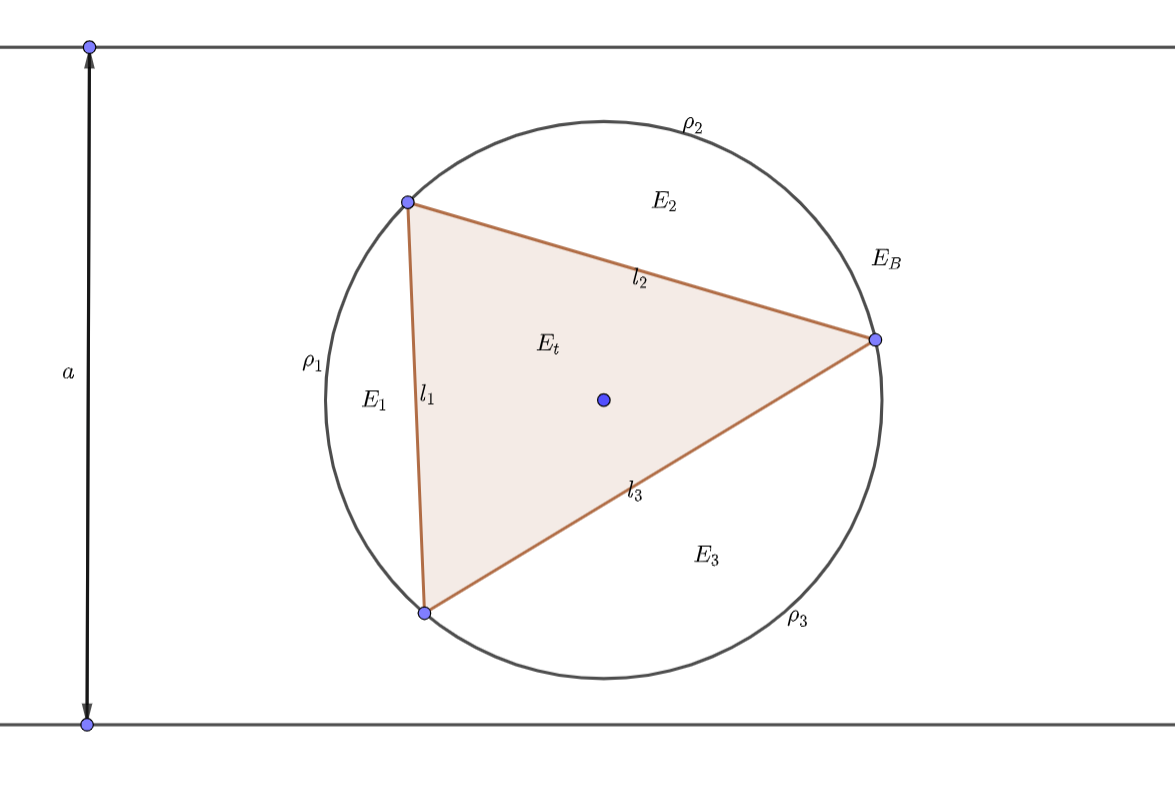
\includegraphics[width=0.8\textwidth]{figure.png}
}
% 表格模板
\renewcommand\arraystretch{0.8} % 设置表格高度为原来的0.8倍
\begin{table}[!htbp] % table标准
    \centering % 表格居中
    \begin{tabular}{p{1cm}<{\centering}p{1cm}<{\centering}p{3cm}<{\centering}p{5cm}<{\centering}} % 设置表格宽度
    %\begin{tabular}{cccc}
        \toprule
        $x_i$ & $f[x_1]$ & $f[x_i,x_{i+1}]$ & $f[x_i,x_{i+1},x_{i+2}]$ \\
        \midrule
        $x_0$ & $f(x_0)$ &                  &                          \\
        $x_0$ & $f(x_0)$ & $f'(x_0)$        &                          \\
        $x_0$ & $f(x_1)$ & $\frac{f(x_1)-f(x_0)}{x_1-x_0}$ & $\frac{f(x_1)-f(x_0)}{(x_1-x_0)^2}-\frac{f'(x_0)}{x_1-x_0}$\\
        \bottomrule
    \end{tabular}
\end{table}

\def\Log{\text{Log}} % 一个简单的宏定义
$\Log$ % 调用方法
\fi

\end{document}